\documentclass[aspectratio=169,11pt,hyperref={colorlinks=true}]{beamer}
\usepackage[utf8]{inputenc}
\usepackage[T1]{fontenc}
\usepackage{fontspec}
\usepackage[absolute,overlay]{textpos}
\usepackage{listingsutf8}
\usepackage{listings-golang}
\usepackage{tikz}
\usepackage{color}
\usepackage{fontawesome5}
\usepackage{svg}


\title{Adopting CDEvents and Embracing Interoperability}
\date[9 May 2023]{cdCon + GitOpsCon | 9 May 2023 | \faTwitter ~@\_cdevents | \faGithub ~cdevents}
\author[Andrea Frittoli]{%
  Andrea Frittoli \\
  Developer Advocate @ IBM\\
  andrea.frittoli@uk.ibm.com \\
  \faTwitter ~@blackchip76 | \faGithub ~afrittoli\\
  ~\\
  Session: \href{https://sched.co/1KUH8}{sched.co/1KUH8}
}

\usetheme{af}

% Code style
\setlststyle

\lstdefinelanguage{koyaml}{
  keywords={github, com, afrittoli, examples, ms, go, helloworld},
  sensitive=false,
  comment=[l]{\#},
  morestring=[b]',
  morestring=[b]"
}

% Automatic section frame
% \AtBeginSection{\frame{\sectionpage}}

\begin{document}

\begin{frame}
\titlepage{}
\end{frame}

\begin{speakerframe}[af_wind.jpg]{Andrea Frittoli}%
  {%
  \faGithub ~afrittoli | \faLinkedin ~andreafrittoli | \faTwitter ~@blackchip76
  }%
  {%
  \begin{itemize}
    \item{Open Source Advocate @ IBM}
    \item{Lives in Wales, enjoys the wind}
    \item{CDEvents maintainer, Events SIG co-chair}
    \item{Chair of CDF Technical Oversight Committee \\ Governing Board}
  \end{itemize}
  }%
\end{speakerframe}

\begin{lpicrblack}[calum-lewis-vA1L1jRTM70-unsplash.jpg]{%
  Photo by \href{https://unsplash.com/@calumlewis}{\underline{Calum Lewis}}, CC0
  }%
  {%
  \tableofcontents
  }%
  {}
  \frametitle{~~~~~~~~~~~~~~~~~~~~~~~~~~~~~~~~~~~~~~~~~~~~~~~~~~~Contents}
\end{lpicrblack}

\section[CDEvents]{A common specification for Continuous Delivery events}

\begin{grayframe}
  \frametitle{Continuous Delivery Pipeline}
  \begin{textblock*}{0.70\paperwidth}(0.15\paperwidth,0.20\paperheight)
    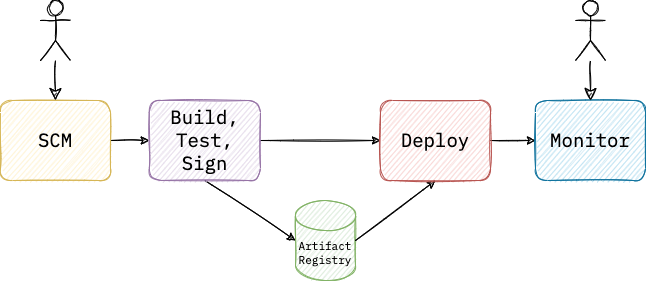
\includegraphics[width=0.70\paperwidth]{img/cdevents-1-no-events.png}
  \end{textblock*}
\end{grayframe}

\begin{grayframe}
  \frametitle{Integrations}
  \begin{textblock*}{0.70\paperwidth}(0.15\paperwidth,0.1\paperheight)
    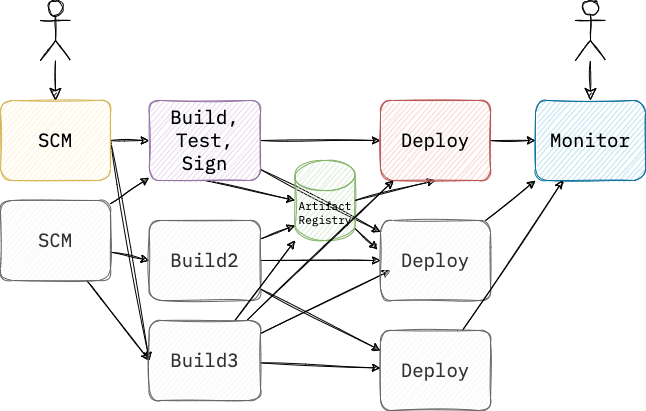
\includegraphics[width=0.70\paperwidth]{img/cdevents-2-no-events-multiple.png}
  \end{textblock*}
\end{grayframe}

\begin{whitetextontwopics}[shutterstock_1044739930.jpg]{%
  % by Igor Bulgarin
  % Shutterstock editorial license: https://support.shutterstock.com/s/article/Premier-Editorial-Content?language=en_US
  % https://www.shutterstock.com/image-photo/dnipro-ukraine-march-12-2018-four-1044739930
  Orchestration
  }{shutterstock_1483333925.jpg}{%
  Choreography
  % by A_Lesik
  % Shutterstock editorial license: https://support.shutterstock.com/s/article/Premier-Editorial-Content?language=en_US
  % https://www.shutterstock.com/image-photo/odessa-ukraine-july22-2019-ballet-classical-1483333925
  }%
  \frametitle{Orchestration vs. Choreography}
\end{whitetextontwopics}

\begin{sectionwithpicmediumcentral}[cdeventscon-gradient-16-9.jpg]{}
\end{sectionwithpicmediumcentral}
\note[itemize]{
  \item How many of you are familiar with CDEvents?
  \item Let's take a step back
  \item Why events in Continuous Delivery?
}

\begin{grayframe}
  \frametitle{Interoperability}
  \begin{textblock*}{0.70\paperwidth}(0.15\paperwidth,0.1\paperheight)
    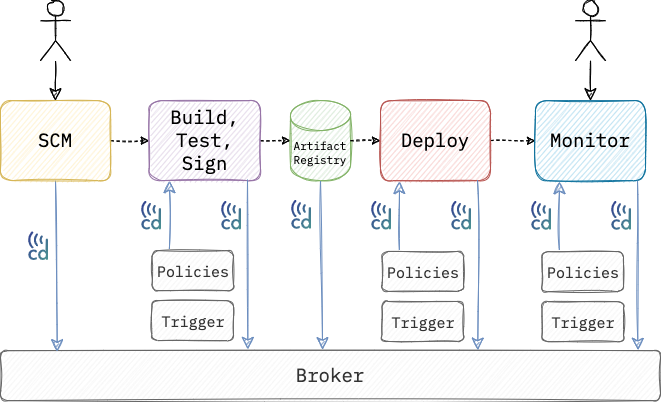
\includegraphics[width=0.70\paperwidth]{img/cdevents-3-events.png}
  \end{textblock*}
\end{grayframe}
\note[itemize]{
  \item Event driven workflows
  \begin{itemize}
    \item Scalable
    \item Decoupled
    \item Flexible
    \item Policy Driven
  \end{itemize}
  \begin{itemize}
    \item Multiple sources to trigger build
    \item Multiple sources to trigger Deployment
    \item Multiple listeners to build events
    \item Policies
  \end{itemize}
}

\begin{textondarkpic}[anthony-yin-okEUu6AMO2Y-unsplash]{%
  Photo by \href{https://unsplash.com/@anthonyin}{\underline{Anthony Yin}}, CC0
  }%
  \frametitle{Observability}
  \begin{itemize}
    \item What's running right now?
    \item What steps were executed?
    \item Where did things go wrong?
    \item How long did it take?
  \end{itemize}
\end{textondarkpic}

\begin{grayframe}
  \frametitle{Interoperability \& Observability}
  \begin{textblock*}{0.80\paperwidth}(0.10\paperwidth,0.15\paperheight)
    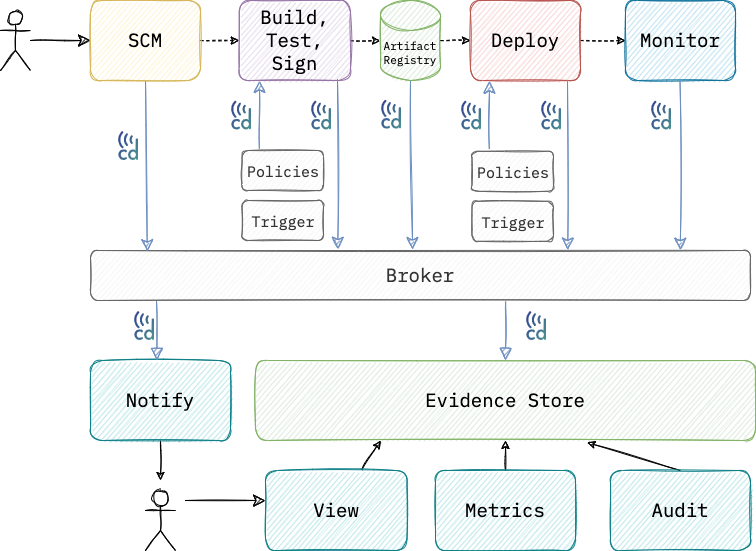
\includegraphics[width=0.80\paperwidth]{img/cdevents-4-interoperability.png}
  \end{textblock*}
\end{grayframe}
\note[itemize]{
  \item Observability of CI/CD pipelines
  \begin{itemize}
    \item Metrics
    \item Notification
    \item Single View
  \end{itemize}
  \item Metrics: unique combinations of tools
  \item Notifications: template to fetch data from multiple sources
  \item Build a diagram, show the need for interoperability
}

\begin{lpicrblack}[whycdevents]{}%
  {%
  \begin{itemize}
    \item Event driven workflows
    \begin{itemize}
      \item Scalable, Decoupled
      \item Flexible
      \item Policy Driven
    \end{itemize}
    \item Observability
    \begin{itemize}
      \item Metrics
      \item Notifications
      \item Single View
    \end{itemize}
    ~ \\
    \textbf{Interoperability!} \\
  \end{itemize}
  }%
  {0.60}
  \frametitle{~~~~~~~~~~~~~~~~~~~~~~~~~~~~~~~~~~~~~~~~~~~~~~~~~~~~~~~~~~~~~~~~~~~~~~~~~Why CDEvents}
\end{lpicrblack}
\note[itemize]{
  Event driven workflows
  \begin{itemize}
    \item Scalable
    \item Decoupled
    \item Flexible
    \item Policy Driven
  \end{itemize}
  Observability of CI/CD pipelines
  \begin{itemize}
    \item Metrics
    \item Notification
    \item Single View
  \end{itemize}
}

\begin{lgrayframerpic}[jon-tyson-FlHdnPO6dlw-unsplash]{%
  Photo by \href{https://unsplash.com/@jontyson}{\underline{Jon Tyson}}, CC0
  }%
  {%
  \begin{itemize}
    \item Interoperability and Events Special Interest Groups
    \item First Commit Oct 2020 
    \item Incubated at the CDF since 2022
  \end{itemize}
  ~\\
  \begin{itemize}
    \item Release v0.1 announced at the CDSummit in Detroit
    \begin{itemize}
      \item Orchestration
      \item Software Configuration Management
      \item Continuous Integration \& Deployment
      \item CloudEvents Binding
      \item Golang SDK
      \item DevOps Metrics
    \end{itemize}
  \end{itemize}
  }%
  {0.65}
  \frametitle{History of CDEvents}
\end{lgrayframerpic}
\note[itemize]{
  \item Incubated at the CDF since 2022
  \item CDEventsCon May 2022
  \item Release v0.1, CDSummit in Detroit, Nov 2022
  \item Scope:
  \begin{itemize}
    \item Orchestration
    \item Software Configuration Management
    \item Continuous Integration
    \item Continuous Deployment
  \end{itemize}
  DevOps Metrics:
  \begin{itemize}
    \item Lead Time for Changes
    \item Deployment Frequency
  \end{itemize}
}

\section{What's New}
\begin{sectionwithpiclargecentral}[josh-sorenson-MjIMc6uhwrE-unsplash.jpg]{Photo by \href{https://unsplash.com/@joshsorenson}{\underline{Josh Sorenson}}, CC0}
\end{sectionwithpiclargecentral}

\begin{tpicstripedframe}%
  {cdevents-banner.png}
  {%
  Incident Events:
  \begin{itemize}
    \item Continuous Operations
    \item Modeled after DORA
    \item Remediation Automation
  \end{itemize}
  }%
  {%
  Test Events:
  \begin{itemize}
    \item Notifications
    \item Test Driven Automation
    \item Metrics
  \end{itemize}
  }%
  {%
  Software Supply Chain Security \\
  \vspace{0.01\textheight}
  \begin{itemize}
    \item Artifact Signed event
    \item Build \& Deployment Automation
  \end{itemize}
  }%
  {%
  Quality of life improvements
  \begin{itemize}
    \item Improved readability
    \item Examples for each event
    \item Refreshed web site
  \end{itemize}
  }%
\end{tpicstripedframe}
\note[itemize]{
  \item Improved readability of the specification
  \item Examples for each event type
  \item Refreshed web site
}

\begin{blackframe}
  \frametitle{SDKs}
  Features:
  \begin{itemize}
    \item JSONSchema Validation
    \item SDK Generated from schemas (Golang)
    \item Improved testing
  \end{itemize}
  ~ \\
  Releases:
  \begin{itemize}
    \item Golang SDK v0.3 released
    \item Java SDK v0.1 (draft) available on maven central
    \item Python SDK v0.1 soon to be on PyPi
  \end{itemize}
\end{blackframe}
\note[itemize]{
  \item Golang SDK v0.3, now generated from JSON schemas
  \item Java SDK published to Maven Central
  \item Python SDK published to PyPi
  \item CDEventer?
}

\section{Tools Adoption}
\begin{sectionwithpiclargecentral}[clay-banks-LjqARJaJotc-unsplash.jpg]{Photo by \href{https://unsplash.com/@claybanks}{\underline{Clay Banks}}, CC0}
\end{sectionwithpiclargecentral}

\begin{3squares}{Overview}{%
    Available:
    \begin{itemize}
      \item Jenkins (plugin published)
      \item Tekton (experimental)
    \end{itemize}
    ~ \\
    ~ \\
    ~ \\
    ~ \\
  }{%
    Work in Progress:
    \begin{itemize}
      \item Spinnaker (RFC approved)
      \item Testkube
    \end{itemize}
    ~ \\
    ~ \\
  }{%
    CNCF Projects:
    \begin{itemize}
      \item Argo
      \item Flux
      \item Harbour
    \end{itemize}
    ~ \\
    ~ \\
    ~ \\
    ~ \\
    Other Projects:
    \begin{itemize}
      \item Tracetest
      \item JReleaser
      \item Shipwright
      \item Jenkins-X
    \end{itemize}
  }
\end{3squares}
\note[itemize]{
  \item Jenkins
  \item Spinnaker
  \item Testkube
  \item Tekton (experimental)
  \item Argo Rollout (PoC)
  \item Flux (PoC)
}

\begin{grayframe}
  \frametitle{Jenkins}
  \begin{textblock*}{0.70\paperwidth}(0.15\paperwidth,0.20\paperheight)
    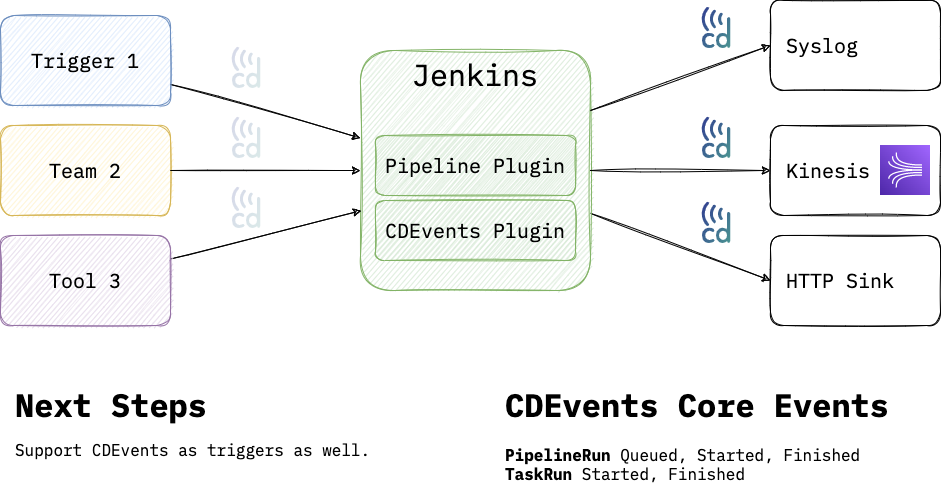
\includegraphics[width=0.70\paperwidth]{img/cdevents-Jenkins.png}
  \end{textblock*}
\end{grayframe}

\begin{blackframe}
  \frametitle{Spinnaker}
  \begin{textblock*}{0.70\paperwidth}(0.15\paperwidth,0.07\paperheight)
    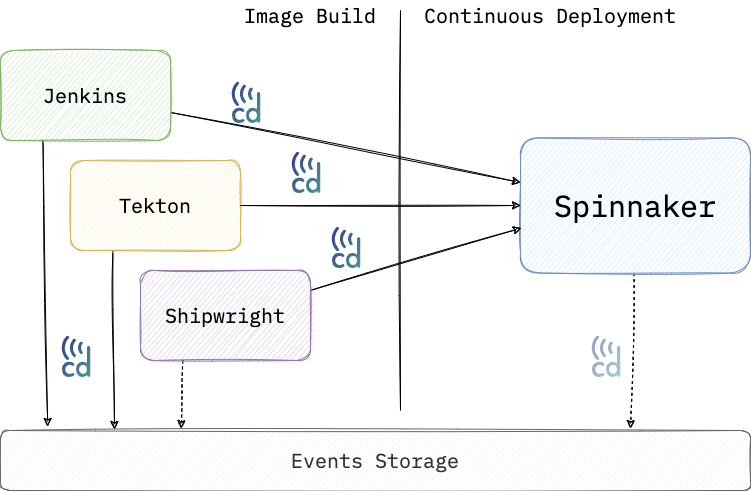
\includegraphics[width=0.70\paperwidth]{img/cdevents-Spinnaker.png}
  \end{textblock*}
\end{blackframe}

\begin{grayframe}
  \frametitle{Testkube}
  \begin{textblock*}{0.70\paperwidth}(0.15\paperwidth,0.20\paperheight)
    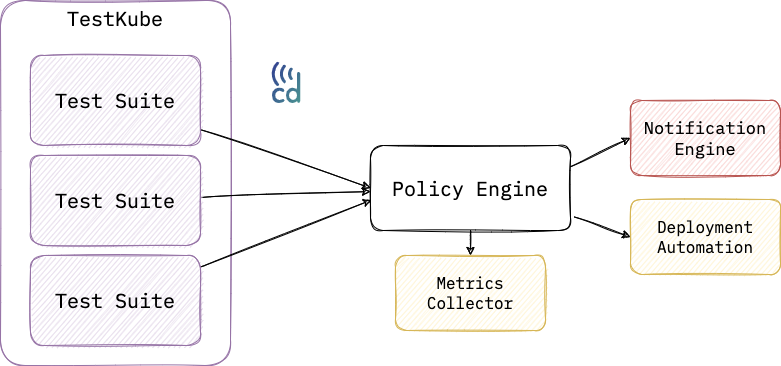
\includegraphics[width=0.70\paperwidth]{img/cdevents-Testkube.png}
  \end{textblock*}
\end{grayframe}

\begin{blackframe}
  \frametitle{Tekton}
  \begin{textblock*}{0.70\paperwidth}(0.15\paperwidth,0.13\paperheight)
    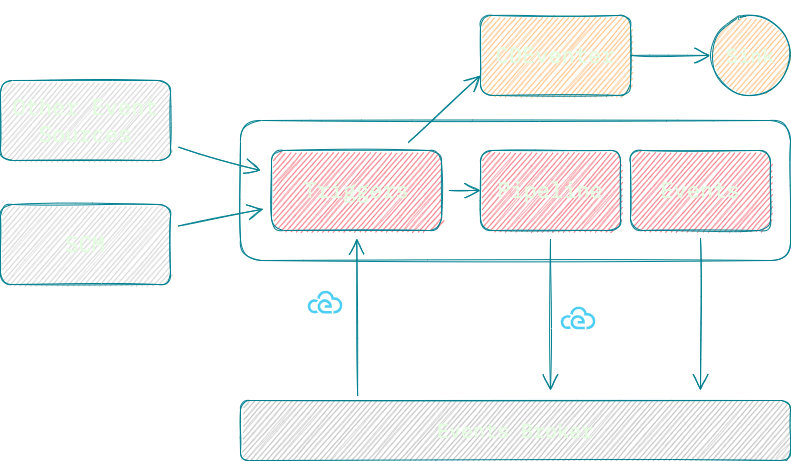
\includegraphics[width=0.70\paperwidth]{img/cdevents-Tekton.png}
  \end{textblock*}
\end{blackframe}
\note[itemize]{
  \item CI Notifications
  \item CD Notifications
  \item Release automation
}

\begin{3squares}{Lessons Learnt}{%
  Adoption:
  \begin{itemize}
    \item Reference Architecture
    \item Event Broker
    \item Responding to events
    \item Incremental adoption
    \item Community
  \end{itemize}
}{%
  Specification:
  \begin{itemize}
    \item Examples events
    \item Example implementations
    \item Generate docs from schema
  \end{itemize}
  ~ \\
}{%
  SDKs:
  \begin{itemize}
    \item Generate SDKs from schema
    \item SDK documentation
    \item SDK validation
    \item JS, Rust
  \end{itemize}
  ~ \\
  ~ \\
  Community:
  \begin{itemize}
    \item CDF, Special Interest Groups
    \item End Users use events today
    \item Collaboration with tool communities
    \item Collaboration with other foundations
  \end{itemize}
}
\end{3squares}

\section{Roadmap}
\begin{sectionwithpiclargecentral}[dimitar-donovski-yrjB4dYWUZU-unsplash.jpg]{Photo by \href{https://unsplash.com/@dmtrdon}{\underline{Dimitar Donovski}}, CC0}
\end{sectionwithpiclargecentral}

\begin{stripedframe}%
  {%
  CDEvents Roadmap \\
  v0.4 and beyond \\
  ~
  }%
  {%
  Supply Chain Security
  \begin{itemize}
    \item SBOM, Provenance
  \end{itemize}
  \begin{itemize}
    \item Signed Events
  \end{itemize}
  }%
  {%
  New features \\
  ~
  \begin{itemize}
    \item Links, Workflow IDs
    \item Compositions
    \item Releases
  \end{itemize}
  }%
  {%
  Software \& Architecture\\
  ~
  \begin{itemize}
    \item SDKs (JS, Rust)
    \item Adapters
    \item Proof of concept
    \item Broker, Policy
  \end{itemize}
  }%
  {%
  Documentation:
  \begin{itemize}
    \item Reference Architecture
    \item Example events
    \item Example implementations
  \end{itemize}
  }%
\end{stripedframe}

\begin{lpicrblack}[nick-fewings-ORSkFfgfEBI-unsplash.jpg]{%
  Photo by \href{https://unsplash.com/@jannerboy62}{\underline{Nick Fewings}}, CC0
  }%
  {%
  \begin{itemize}
    \item CDF, SIG Interop:\\
    Reference Architecture
  \end{itemize}
  ~ \\
  \begin{itemize}
    \item CNCF TAG App Delivery
  \end{itemize}
  ~ \\
  \begin{itemize}
    \item Value Stream Management\\
          Interoperability (VSMI) TC
  \end{itemize}
  ~ \\
  \begin{itemize}
    \item CDF, Workshop working group
  \end{itemize}
  }%
  {0.35}
  \frametitle{~~~~~~~~~~~~~~~~~~~~~~~~~~~~~~~~~~~~~~~~~~~~~~~~~~~Collaborations}
\end{lpicrblack}

\begin{stripedframe}%
  {%
  Community
  ~ \\
  ~ \\
  }%
  {%
  CDF \\
  ~
  \begin{itemize}
    \item SIG Interop
    \item SIG Supply Chain
    \item SIG Best Practices
  \end{itemize}
  }%
  {%
  Tools communities \\
  ~
  \begin{itemize}
    \item Tekton
    \item Spinnaker
    \item Shipwright
    \item Jenkins
    \item Jenkins X
    \item Flux, Argo
  \end{itemize}
  }%
  {%
  Companies \\
  ~
  \begin{itemize}
    \item Ericsson
    \item IBM / RedHat
    \item Apple
    \item VMWare
    \item Fidelity
    \item SAS
  \end{itemize}
  }%
  {%
  Get Involved!! \\
  ~
  \begin{itemize}
    \item Specification
    \item SDKs (Rust, JS, Ruby, C\#)
    \item Tools
    \item Proof-of-concepts
    \item End users
  \end{itemize}
  }%
\end{stripedframe}

\section[Thank You]{Thank You!}

\begin{sectionwithpiclargecentral}[carl-jorgensen-5nrnxx_tWe8-unsplash.jpg]{Brecon Beacons, Walse, Photo by \href{https://unsplash.com/@scamartist}{\underline{Carl Jorgensen}}, CC0}
\end{sectionwithpiclargecentral}

\begin{blackframe}
  \frametitle{References}
  \begin{itemize}
    \item \href{https://cdevents.dev}{cdevents.dev, github.com/cdevents}
    \item \href{https://github.com/cdevents/spec/blob/main/CDEvents_Whitepaper.pdf}{github.com/cdevents/spec/blob/main/CDEvents\_Whitepaper.pdf} \\~
    \item \href{https://github.com/jenkinsci/cdevents-plugin}{github.com/jenkinsci/cdevents-plugin}
    \item \href{https://github.com/spinnaker/governance/blob/master/rfc/cdevents-spinnaker.md}{github.com/spinnaker/governance/blob/master/rfc/cdevents-spinnaker.md}
    \item \href{https://github.com/afrittoli/cdeventer}{github.com/afrittoli/cdeventer} \\~
    \item \href{https://github.com/cncf/tag-app-delivery}{github.com/cncf/tag-app-delivery}
    \item \href{https://www.oasis-open.org/committees/tc_home.php?wg_abbrev=vsmi}{VSMI TC @ www.oasis-open.org/committees}
  \end{itemize}
  ~\\
  ~\\
  Andrea Frittoli | \href{mailto:andrea.frittoli@uk.ibm.com}{andrea.frittoli@uk.ibm.com} \\
  \faTwitter ~@blackchip76 | \faGithub ~afrittoli | \faLinkedin ~andreafrittoli
\end{blackframe}

\end{document}
